\chapter{Data}

\section{Data structure}
This thesis will cover a rather large (at least in the machine learning sense) climate data set. The data set covers two time periods; the "historical" period, spanning from 1951 till 2015, and the "future" data set, spanning from 2015 till 2100. In the data we find "images" of the climate, each image contains a number of \glspl{channel}, which covers one climatological variable each. One "image" spans one day, and contains aggregated data from that day (either minimum, mean, or maximum).

\subsection{Climate models}
The machine learning task in this thesis is of course \gls{downscaling}, which means that data must exist in two different resolutions. In this case, the two resolutions are populated by two different climate models. The low-resolution data is created by the EC-Earth-3 \gls{gcm}, while the high-resolution data is created by the HCLIM \gls{ddm}. 

Naturally, the two climate models operate on two different grid projections. While the EC-Earth-3 data is on a regular latitude-longitude grid,the HCLIM data uses a rotated polar grid. As the two projections map the Earth in wildly different manners, the EC-Earth-3 data set has to cover a much bigger area, than the HCLIM data, to make sure that it encompasses all the of the HCLIM area. The domains of the two datasets have been visualized in \autoref{fig:domains}.

\begin{figure}
    \centering
    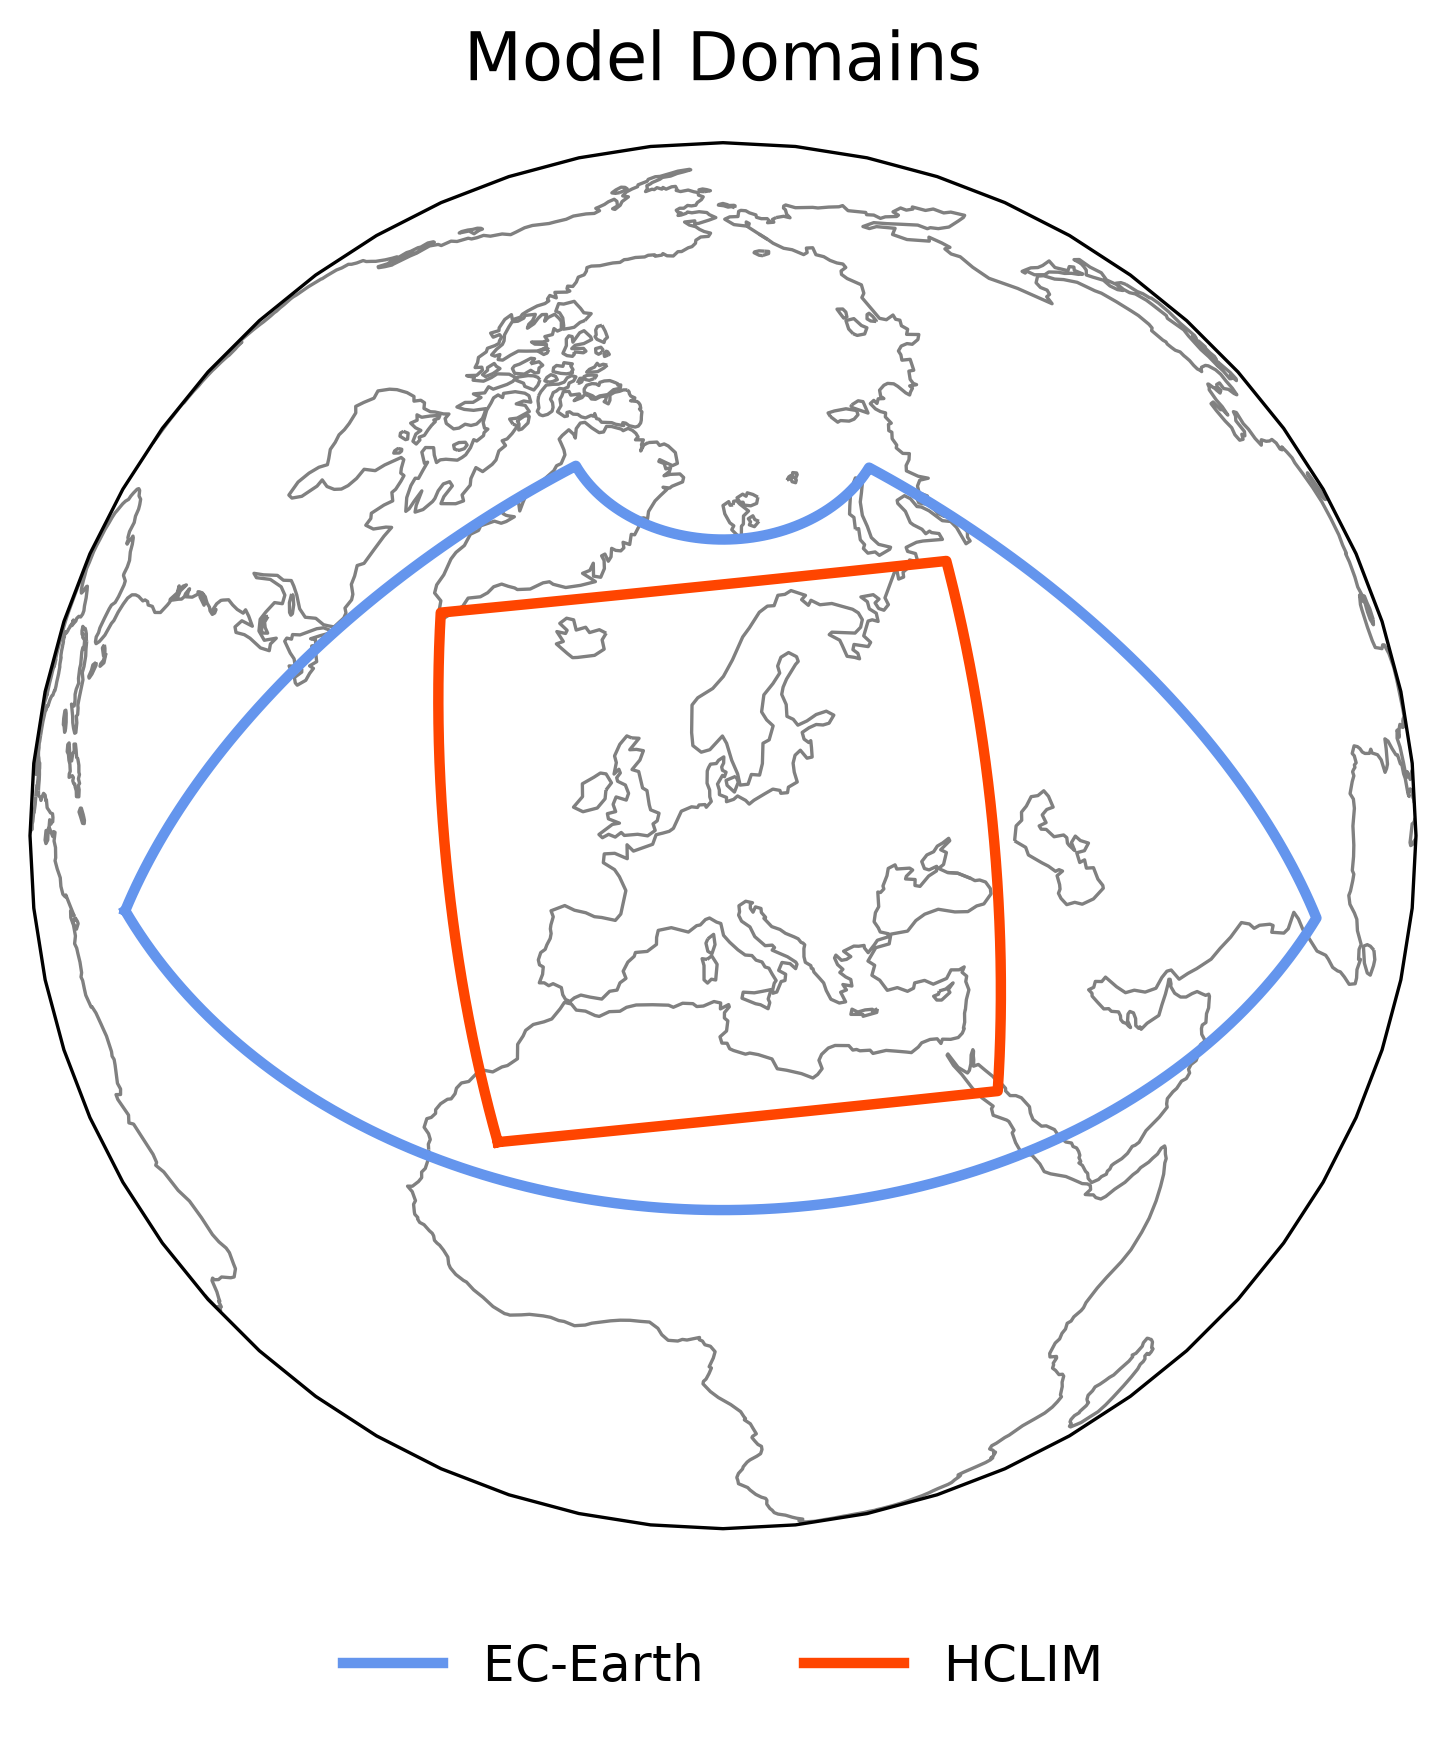
\includegraphics[width=0.5\linewidth]{figures/data_section/domains.png}
    \caption{Spatial areas of the two climate model datasets. The blue line represents the outer edge of the EC-Earth-3 (\gls{gcm}) data, and the orange-red line represents the outer edge of the HCLIM (\gls{ddm}) data}
    \label{fig:domains}
\end{figure}

In climate science, a climate model is a numerical estimator, which takes satellite data as input, as well as a set of hyperparameters, and uses an expensive physics-based method to calculate how the climate looks on three-dimensional grid (two spatial dimensions and one temporal). In other words, the models take the measured data and estimates how the corresponding climate look on the entire planet, while also estimating a number of years into the future. As the models are highly dependant on their initialisation it is customary to run several \glspl{realisation} to model the climate in a less biased fashion. To make sure, that such internal variation is accounted for, this data set includes 3 \glspl{realisation} for both the historical data, and both scenarios

\subsection{Scenarios} \label{sec:scenarios}
In the future period, for both data sets, there are two \glspl{scenario}; "SSP126" and "SSP370". SSP is short for "Shared Socioeconomic Pathways" and they describe different versions of how much emission is produced until the year 2100. SSP126 is on the mild, green side of the spectrum, modelling a more sustainable future, where the excess energy on earth eventually declines as the human race start correcting their mistakes. SSP370 is a more conservative estimate, in which the emission level will rise every year, rapidly heating up the planet.

A visualisation  of the data structure can be found in \autoref{fig:data_structure}.

\begin{figure}
    \centering
    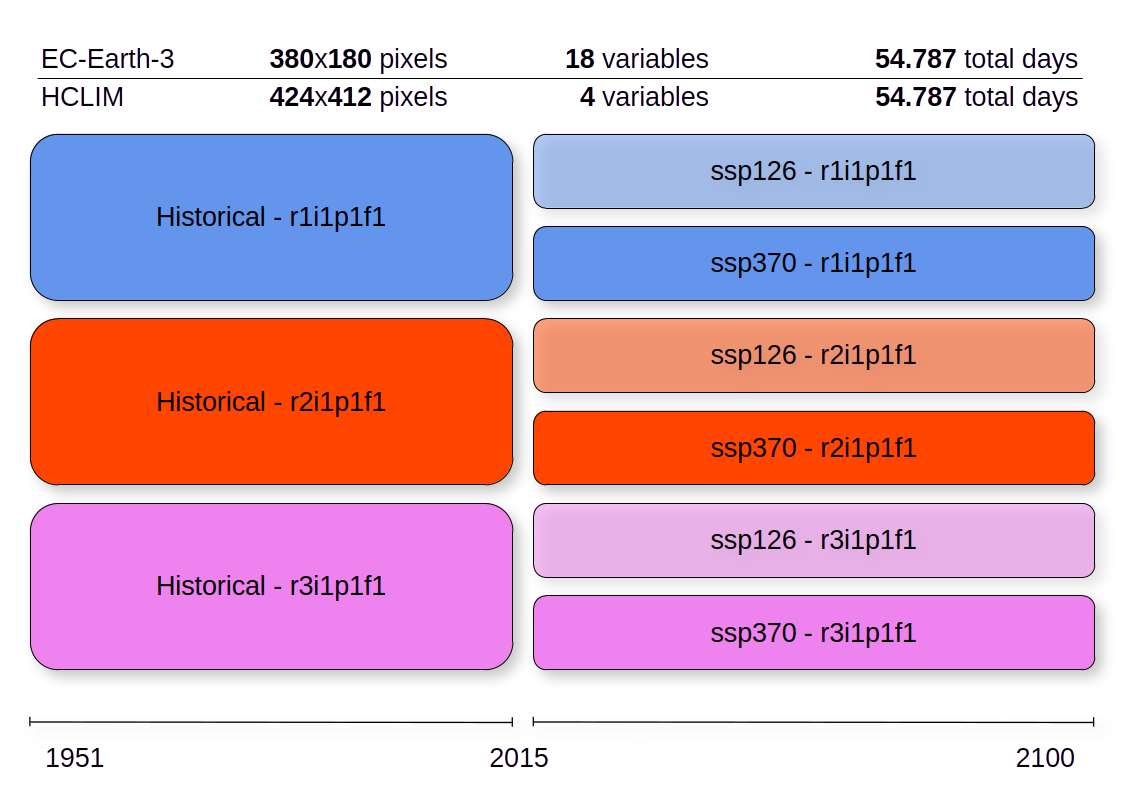
\includegraphics[width=0.8\linewidth]{figures/data_section/data_structure.png}
    \caption{Data structure of the EC-Earth-3 and HCLIM data pair. It features two realisations for each of the two scenarios and the historical data. EC-Earth has a resolution of 380x180 pixels and 18 variables, while HCLIM has 424x412 and 4 variables. I amounts to a total of 499.074.007.488 pixel value climate estimates}
    \label{fig:data_structure}
\end{figure}

\subsection{Static data}
Besides the two climate models, there are also two static features. In this sense "static" means that these features do not change over the temporal dimension. The two variables are "Orography", which describes the topography of the target area, and a "Land-Water mask" which describes the ratio of the grid point covered by water. Both features are delivered at a resolution matching the target grid.

\subsection{Variables}
As mentioned in \autoref{sec:scenarios} the EC-Earth-3 and HCLIM data has 18 and 4 variables respectively. In this case there are two types of variables, single-level variables and pressure-level variables. Single-level variables are only recorded once and typically model surface level climate like 2 meter temperature or precipitation. Pressure-level variables are recorded on several levels of the atmosphere. In this data we are working with three different pressure levels 500, 700, and 850 hPa, and on each level we see variables like pressure, humidity, etc. See \autoref{tab:variables} for full list of variables. 

\begin{table}[] \label{tab:variables}
    \centering
    \begin{tabular}{l|l|l|l}
        \multicolumn{3}{l}{\textbf{Single-level Variables}} \\ \toprule
        \underline{TAS}     & Temperature At Surface (2m)   & Kelvin                & 380x180 and 424x412 \\ \midrule
        \underline{TASMAX}  & Daily max TAS                 & Kelvin                & 380x180 and 424x412 \\ \midrule
        \underline{TASMIN}  & Daily min TAS                 & Kelvin                & 380x180 and 424x412 \\ \midrule
        \underline{PR}      & Precipitation                 & $\frac{kg}{m^2 s}$    & 380x180 and 424x412 \\ \midrule
        CLT                 & Cloud Area Fraction           & \%                    & 380x180 \\ \midrule
        PSL                 & Sea Level Pressure            & Pascal                & 380x180 \\ \midrule
        \multicolumn{3}{l}{\textbf{Pressure-level Variables} (500 hPa, 700 hPa, 850 hPa} \\ \toprule
        UA                  & Eastward Wind                 & $m/s$                 & 380x180 \\ \midrule
        VA                  & Northward Wind                &  $m/s$                & 380x180 \\ \midrule
        HUS                 & Specific Humidity             & Watermass / Airmass   & 380x180 \\ \midrule
        TA                  & Air Temperature               & Kelvin                & 380x180 \\ \midrule
        \multicolumn{3}{l}{\textbf{Static variables}} \\ \toprule
        Orog                & Orography                     & m                     & 424x412 \\ \midrule
        SFTLF               & Sea Fraction to Land Fraction & \%                    & 424x412 \\ \midrule
    \end{tabular}
    \caption{Table of variables in dataset. Underlined variables are additionally used in as target data (albeit in a higher resolution)}
    \label{tab:placeholder}
\end{table}

\section{Data distribution}
In this section I will analyse the distributions and temporal developments of the data to develop an understanding of how the climate data can be modelled. This analysis is done prior to creating the model in order to best create preprocessing flows, that match the model capabilities and functions.

\subsection{Time-series data}
To start off let's have a look at the temporal development of the data. Specifically, let's model how the different \glspl{realisation} and \glspl{scenario} develop over time. This will help develop the understanding of the climate impact on temperature and precipitation through time. In the end, this will help us design the experiments and split data correctly.


\newpage
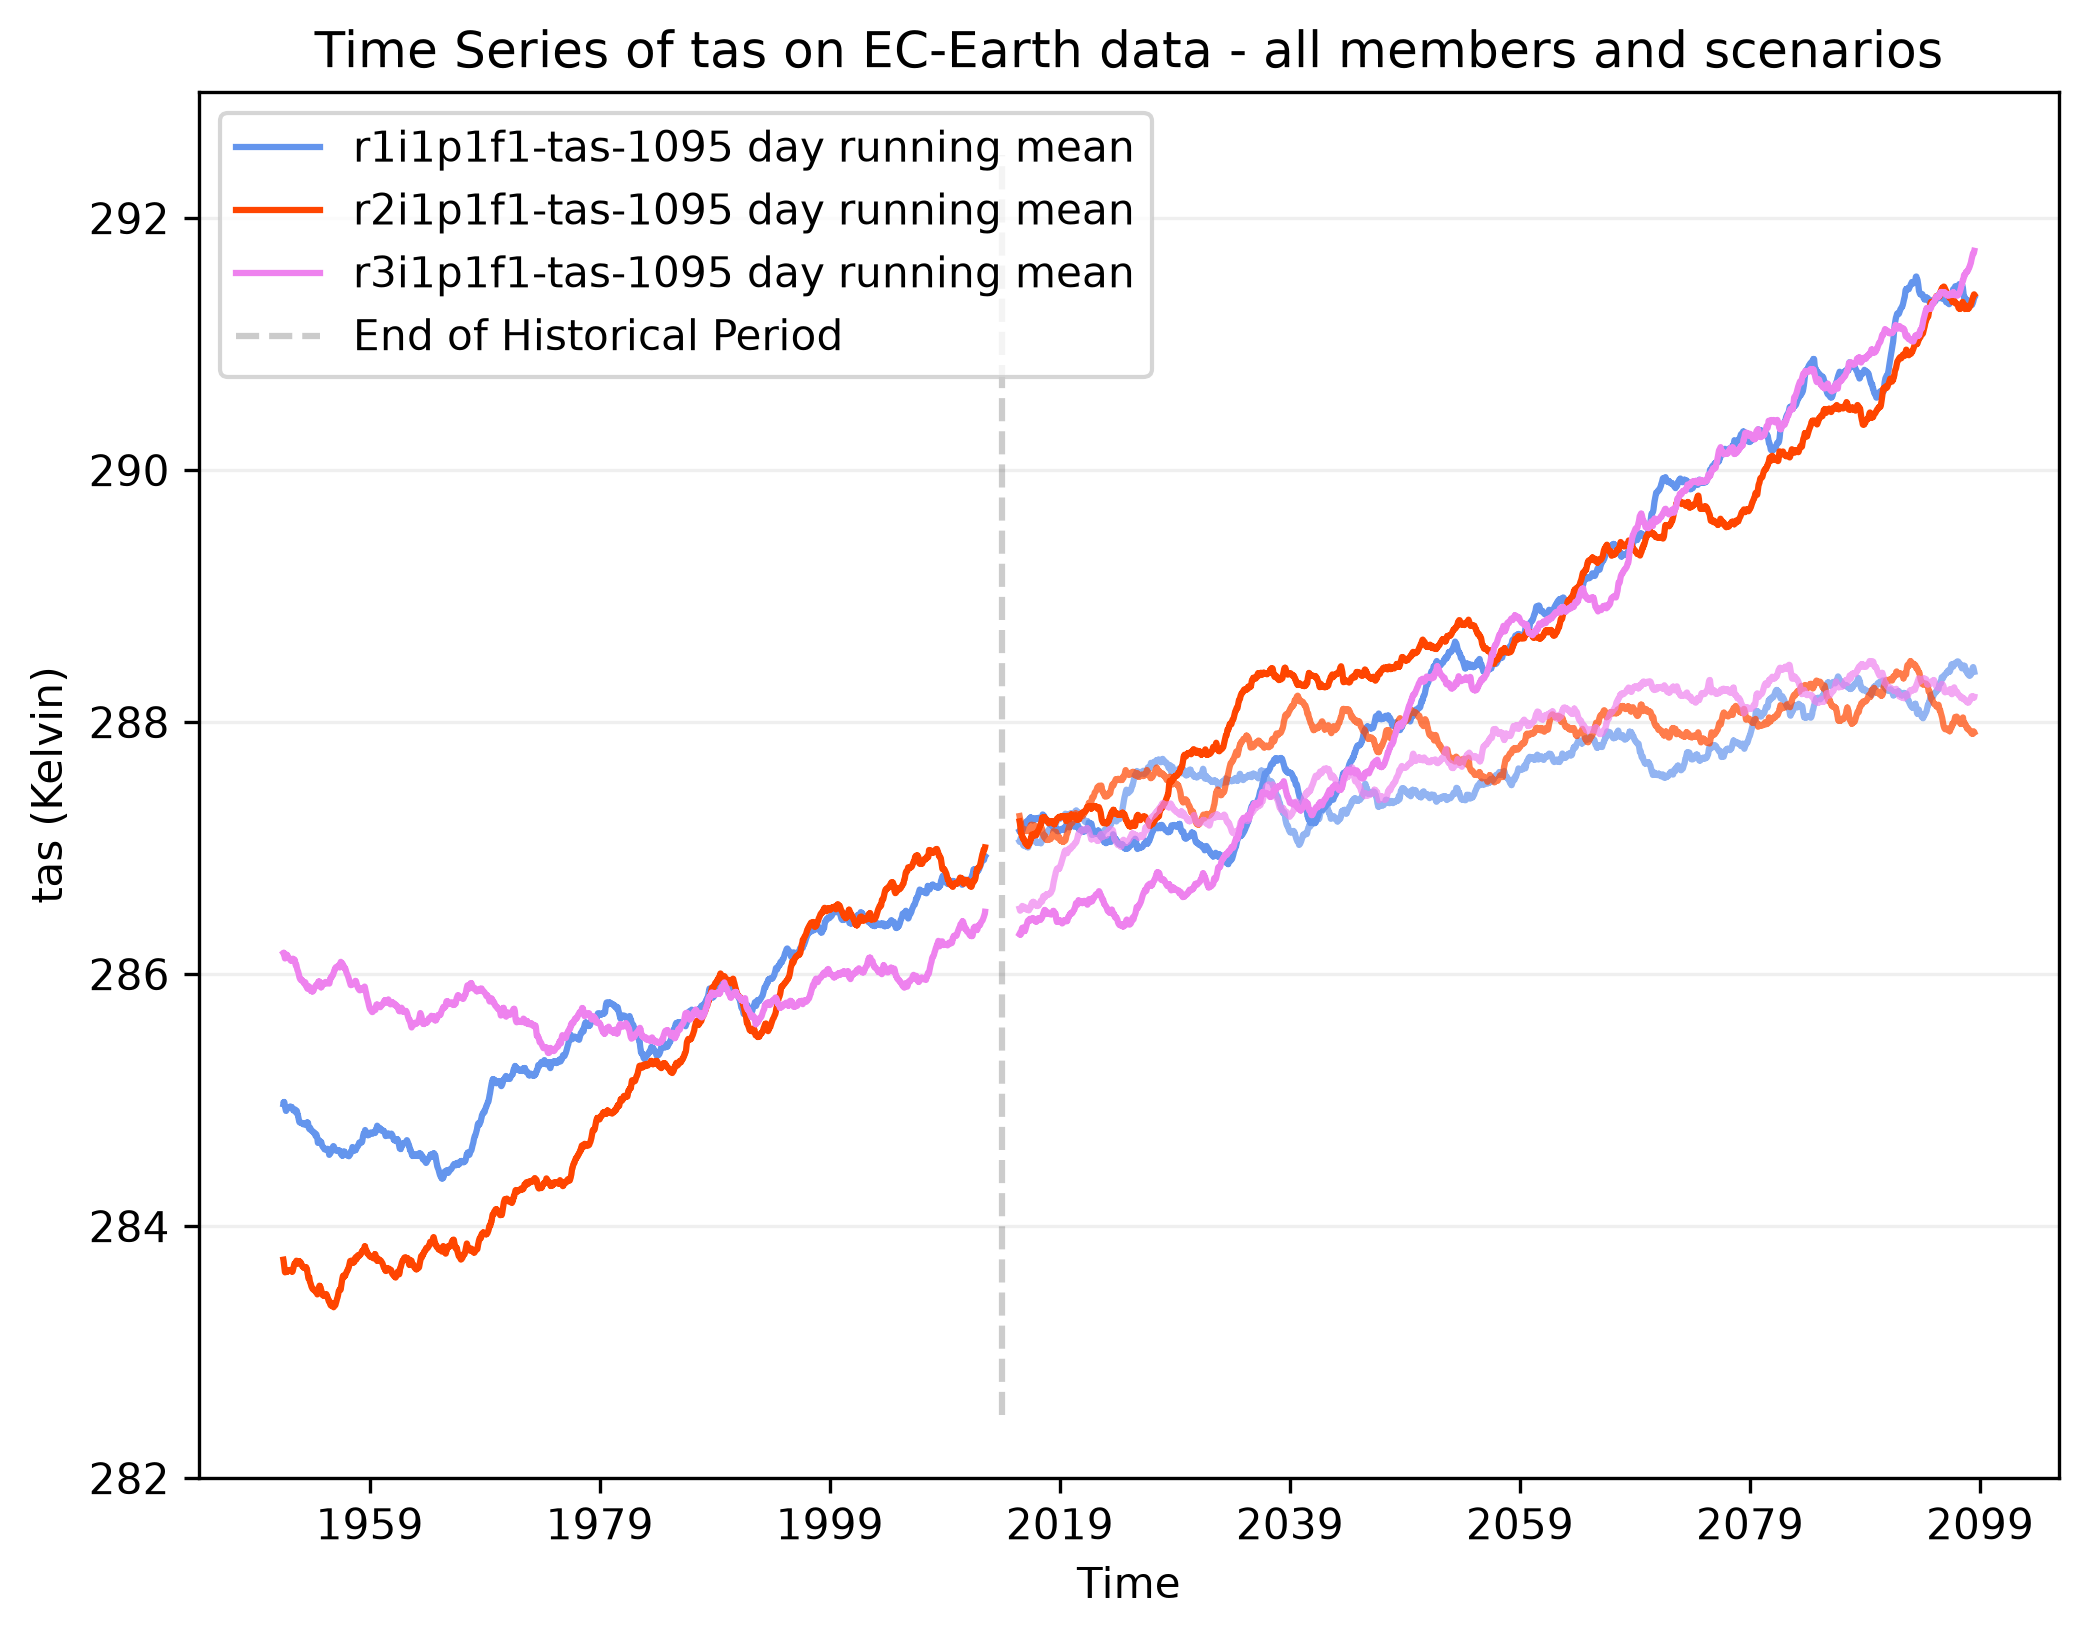
\includegraphics[width=1\linewidth]{figures/data_section/climatology/timeseries_tas.png}
\newpage
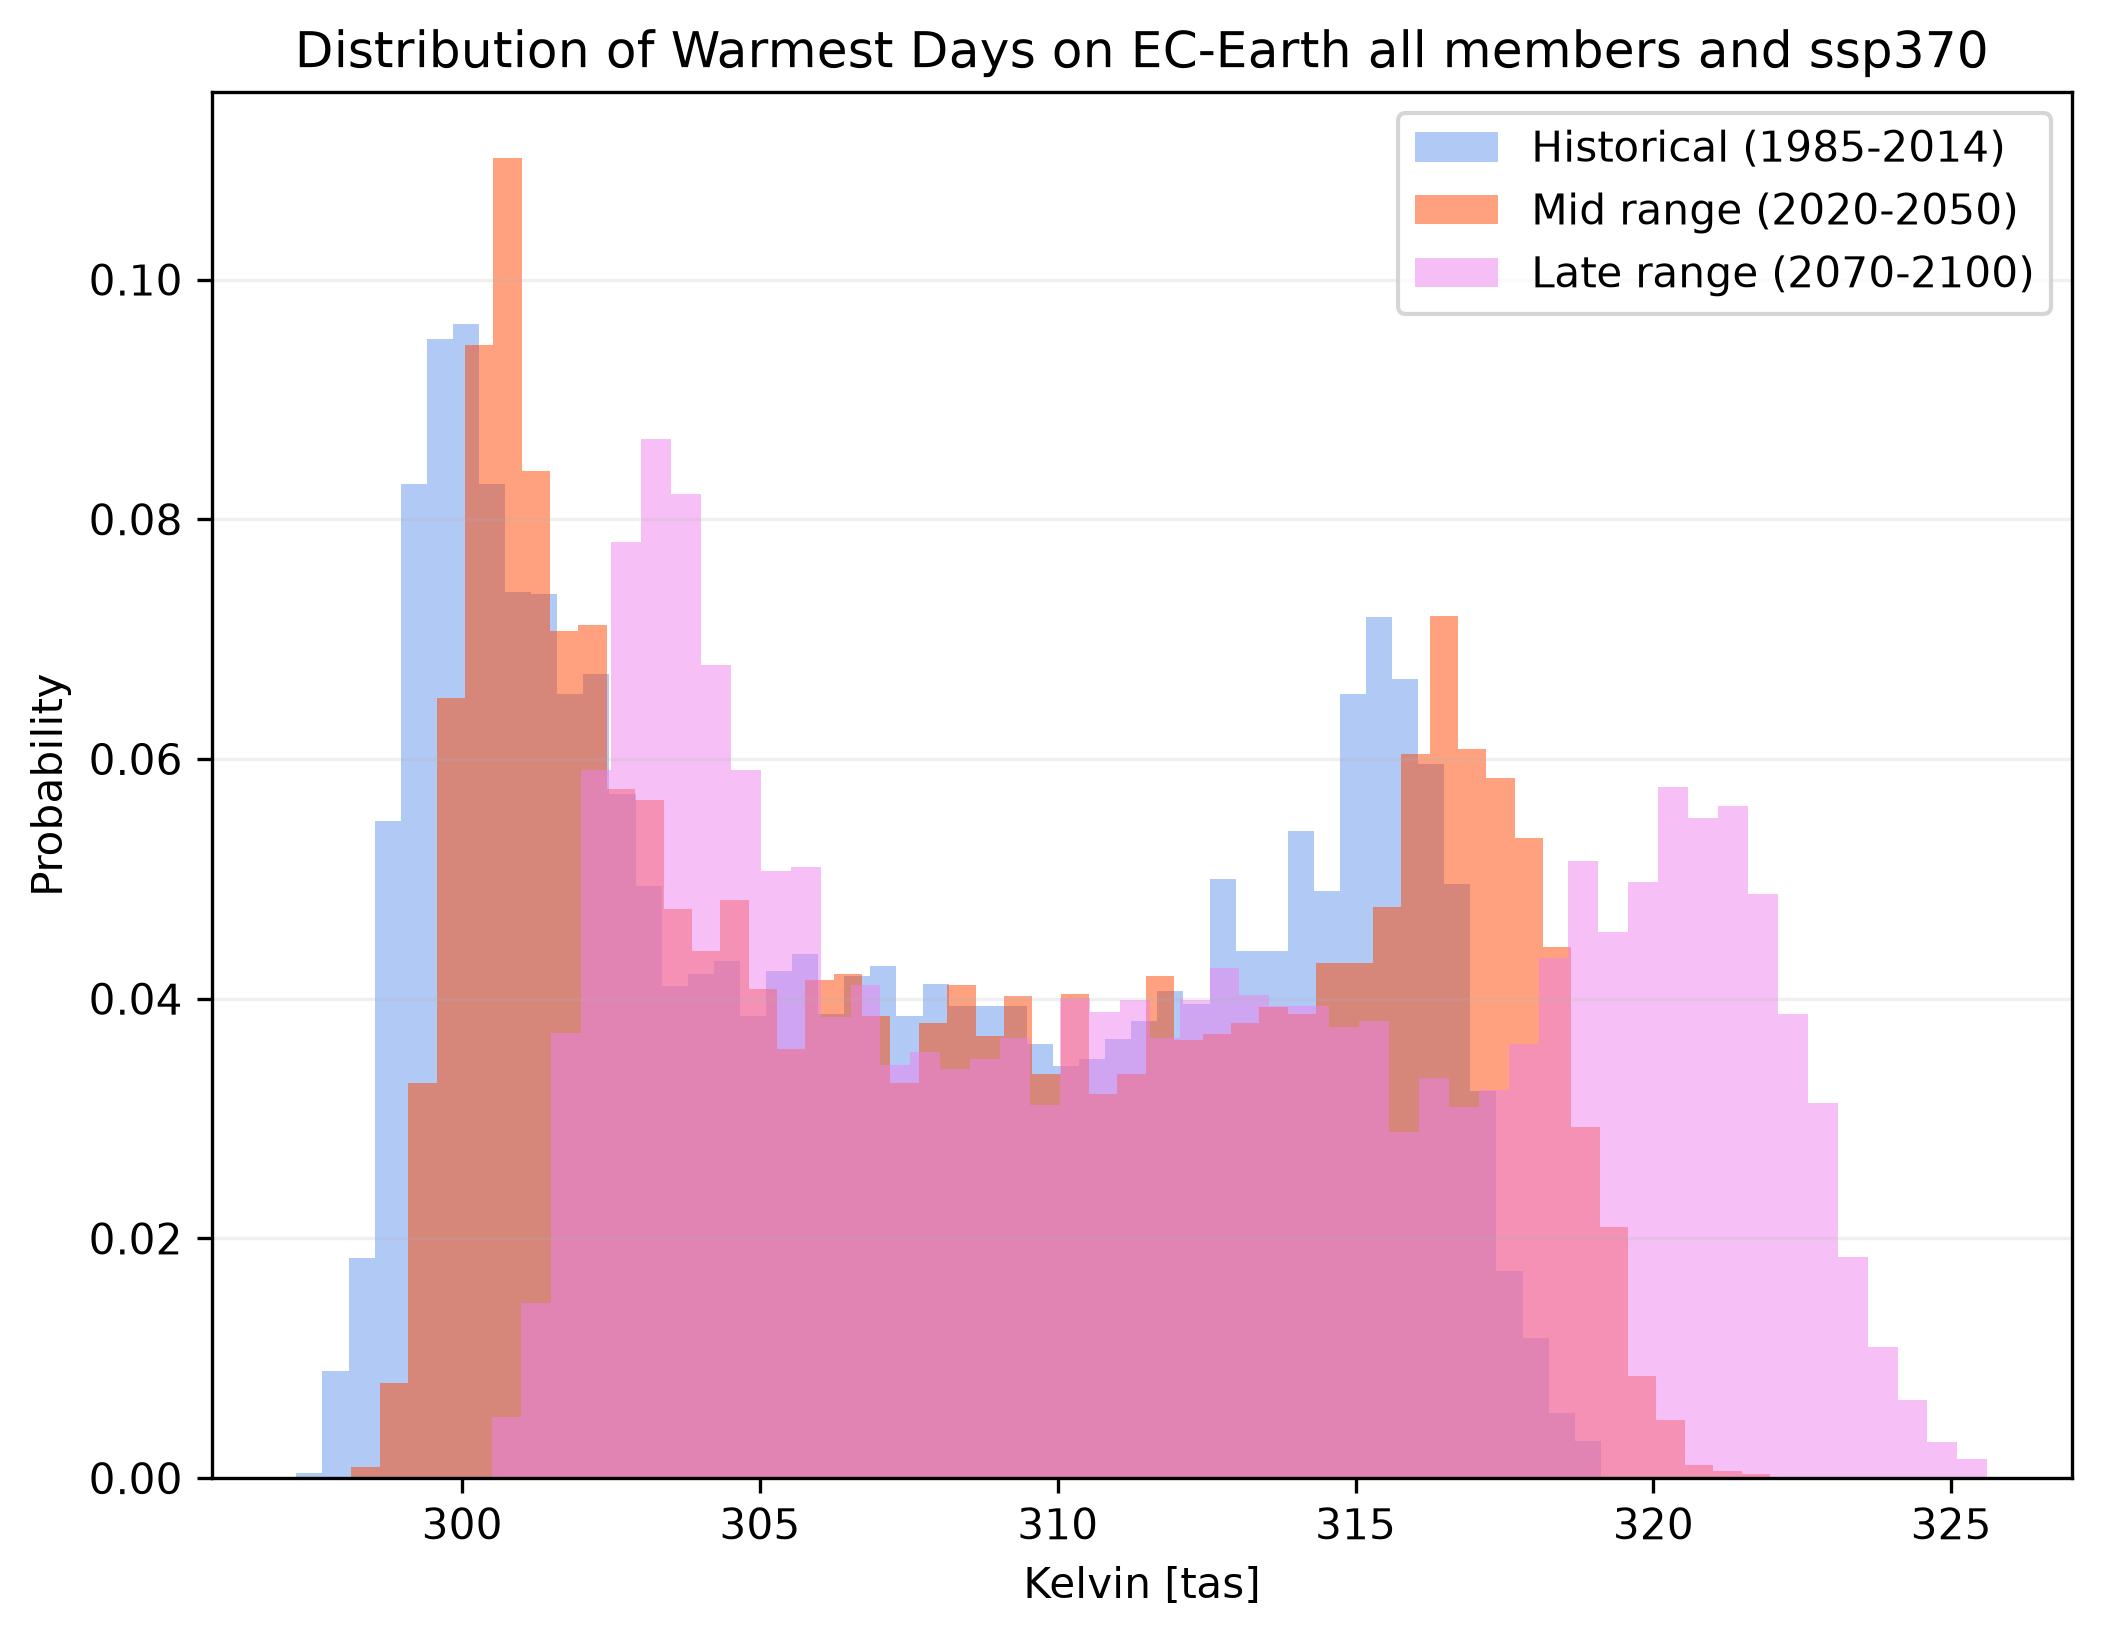
\includegraphics[width=1\linewidth]{figures/data_section/climatology/max_tas_days.png}
\newpage
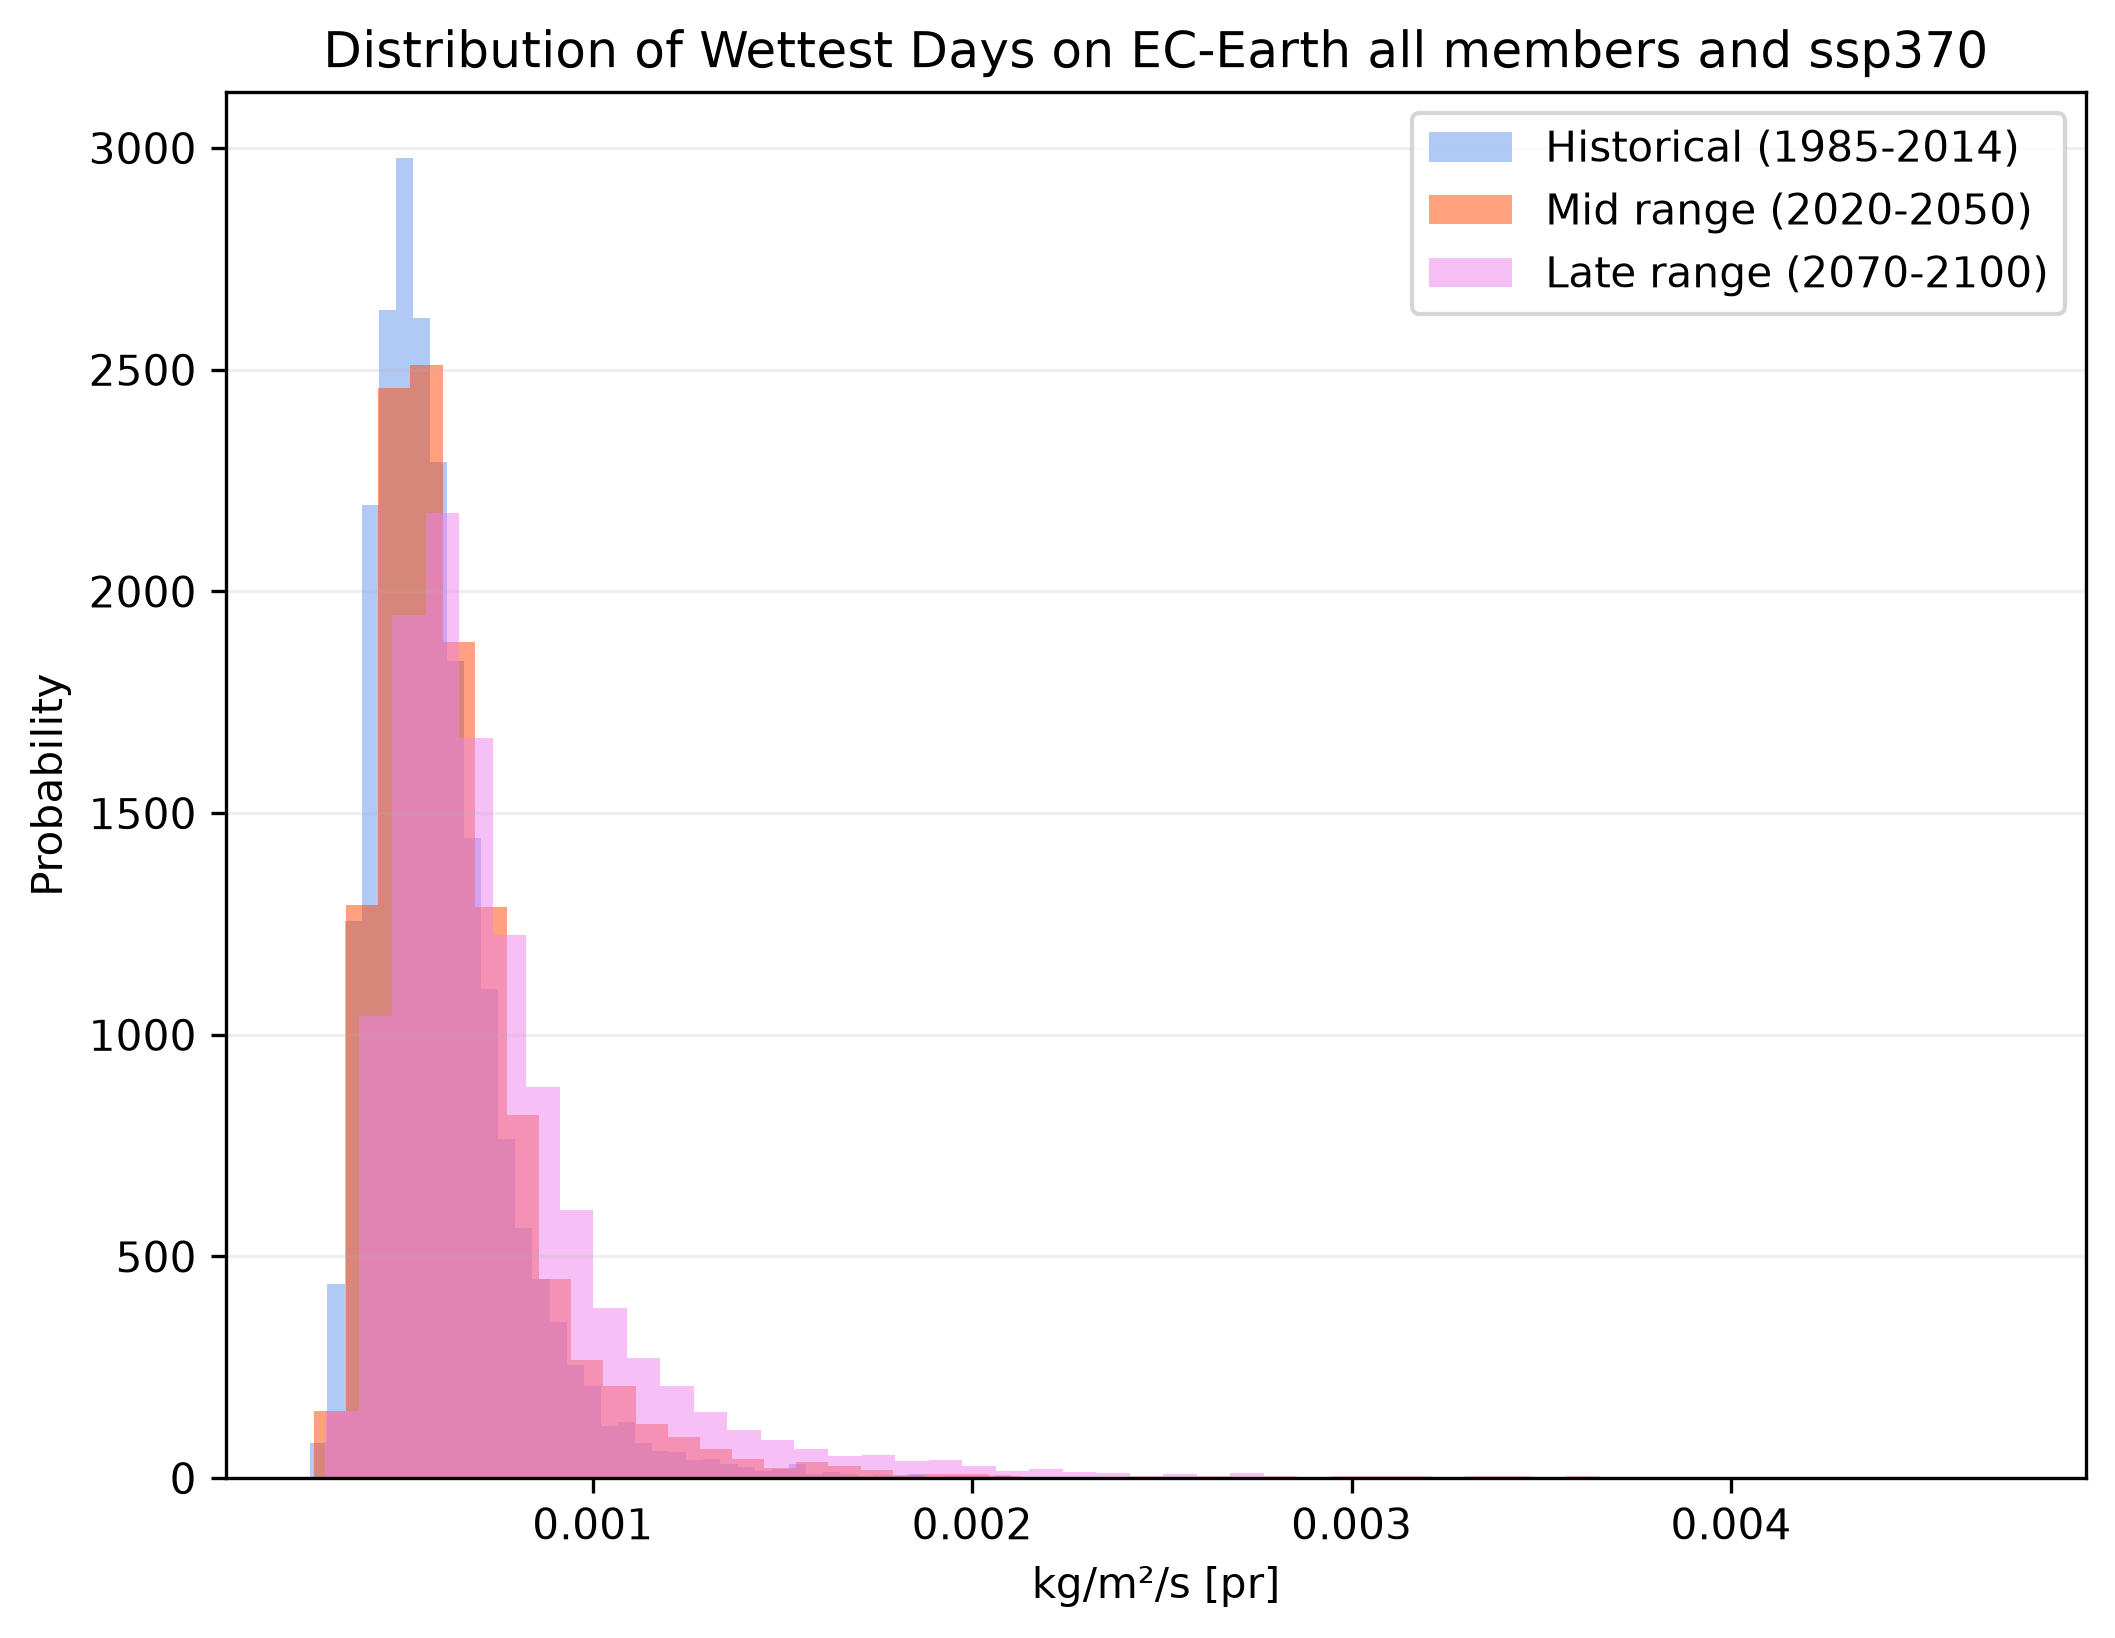
\includegraphics[width=1\linewidth]{figures/data_section/climatology/max_pr_days.png}
\newpage
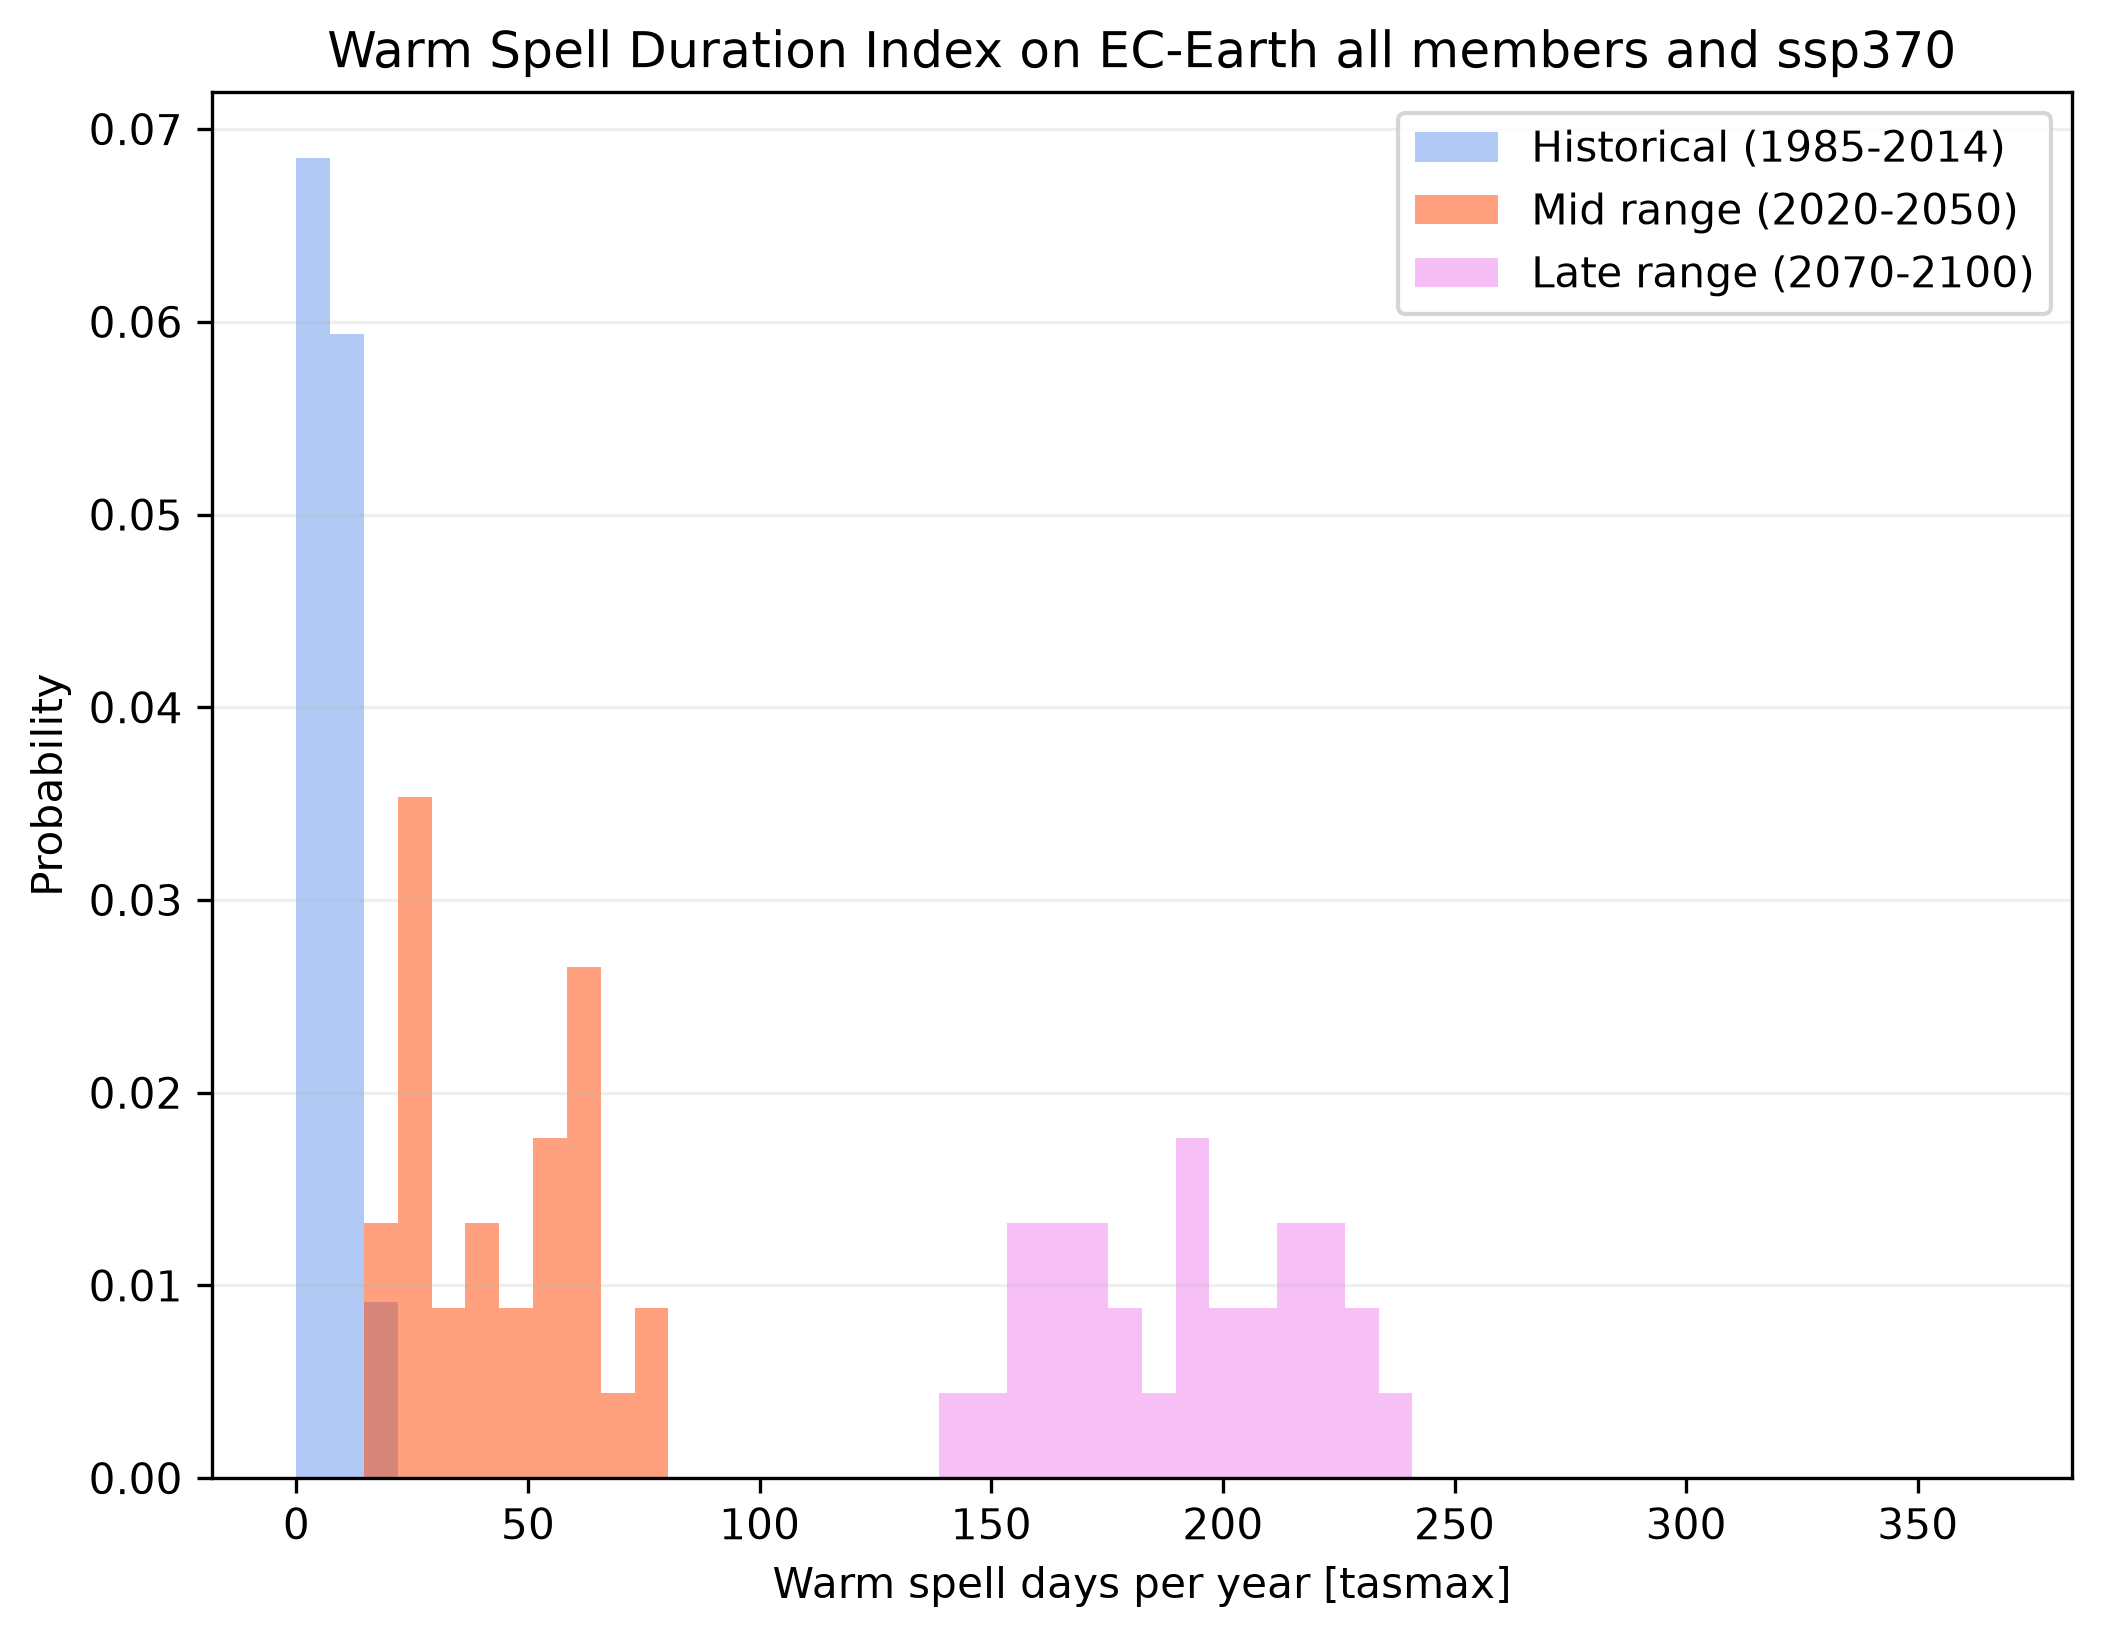
\includegraphics[width=1\linewidth]{figures/data_section/climatology/warm_spell_days.png}
\newpage
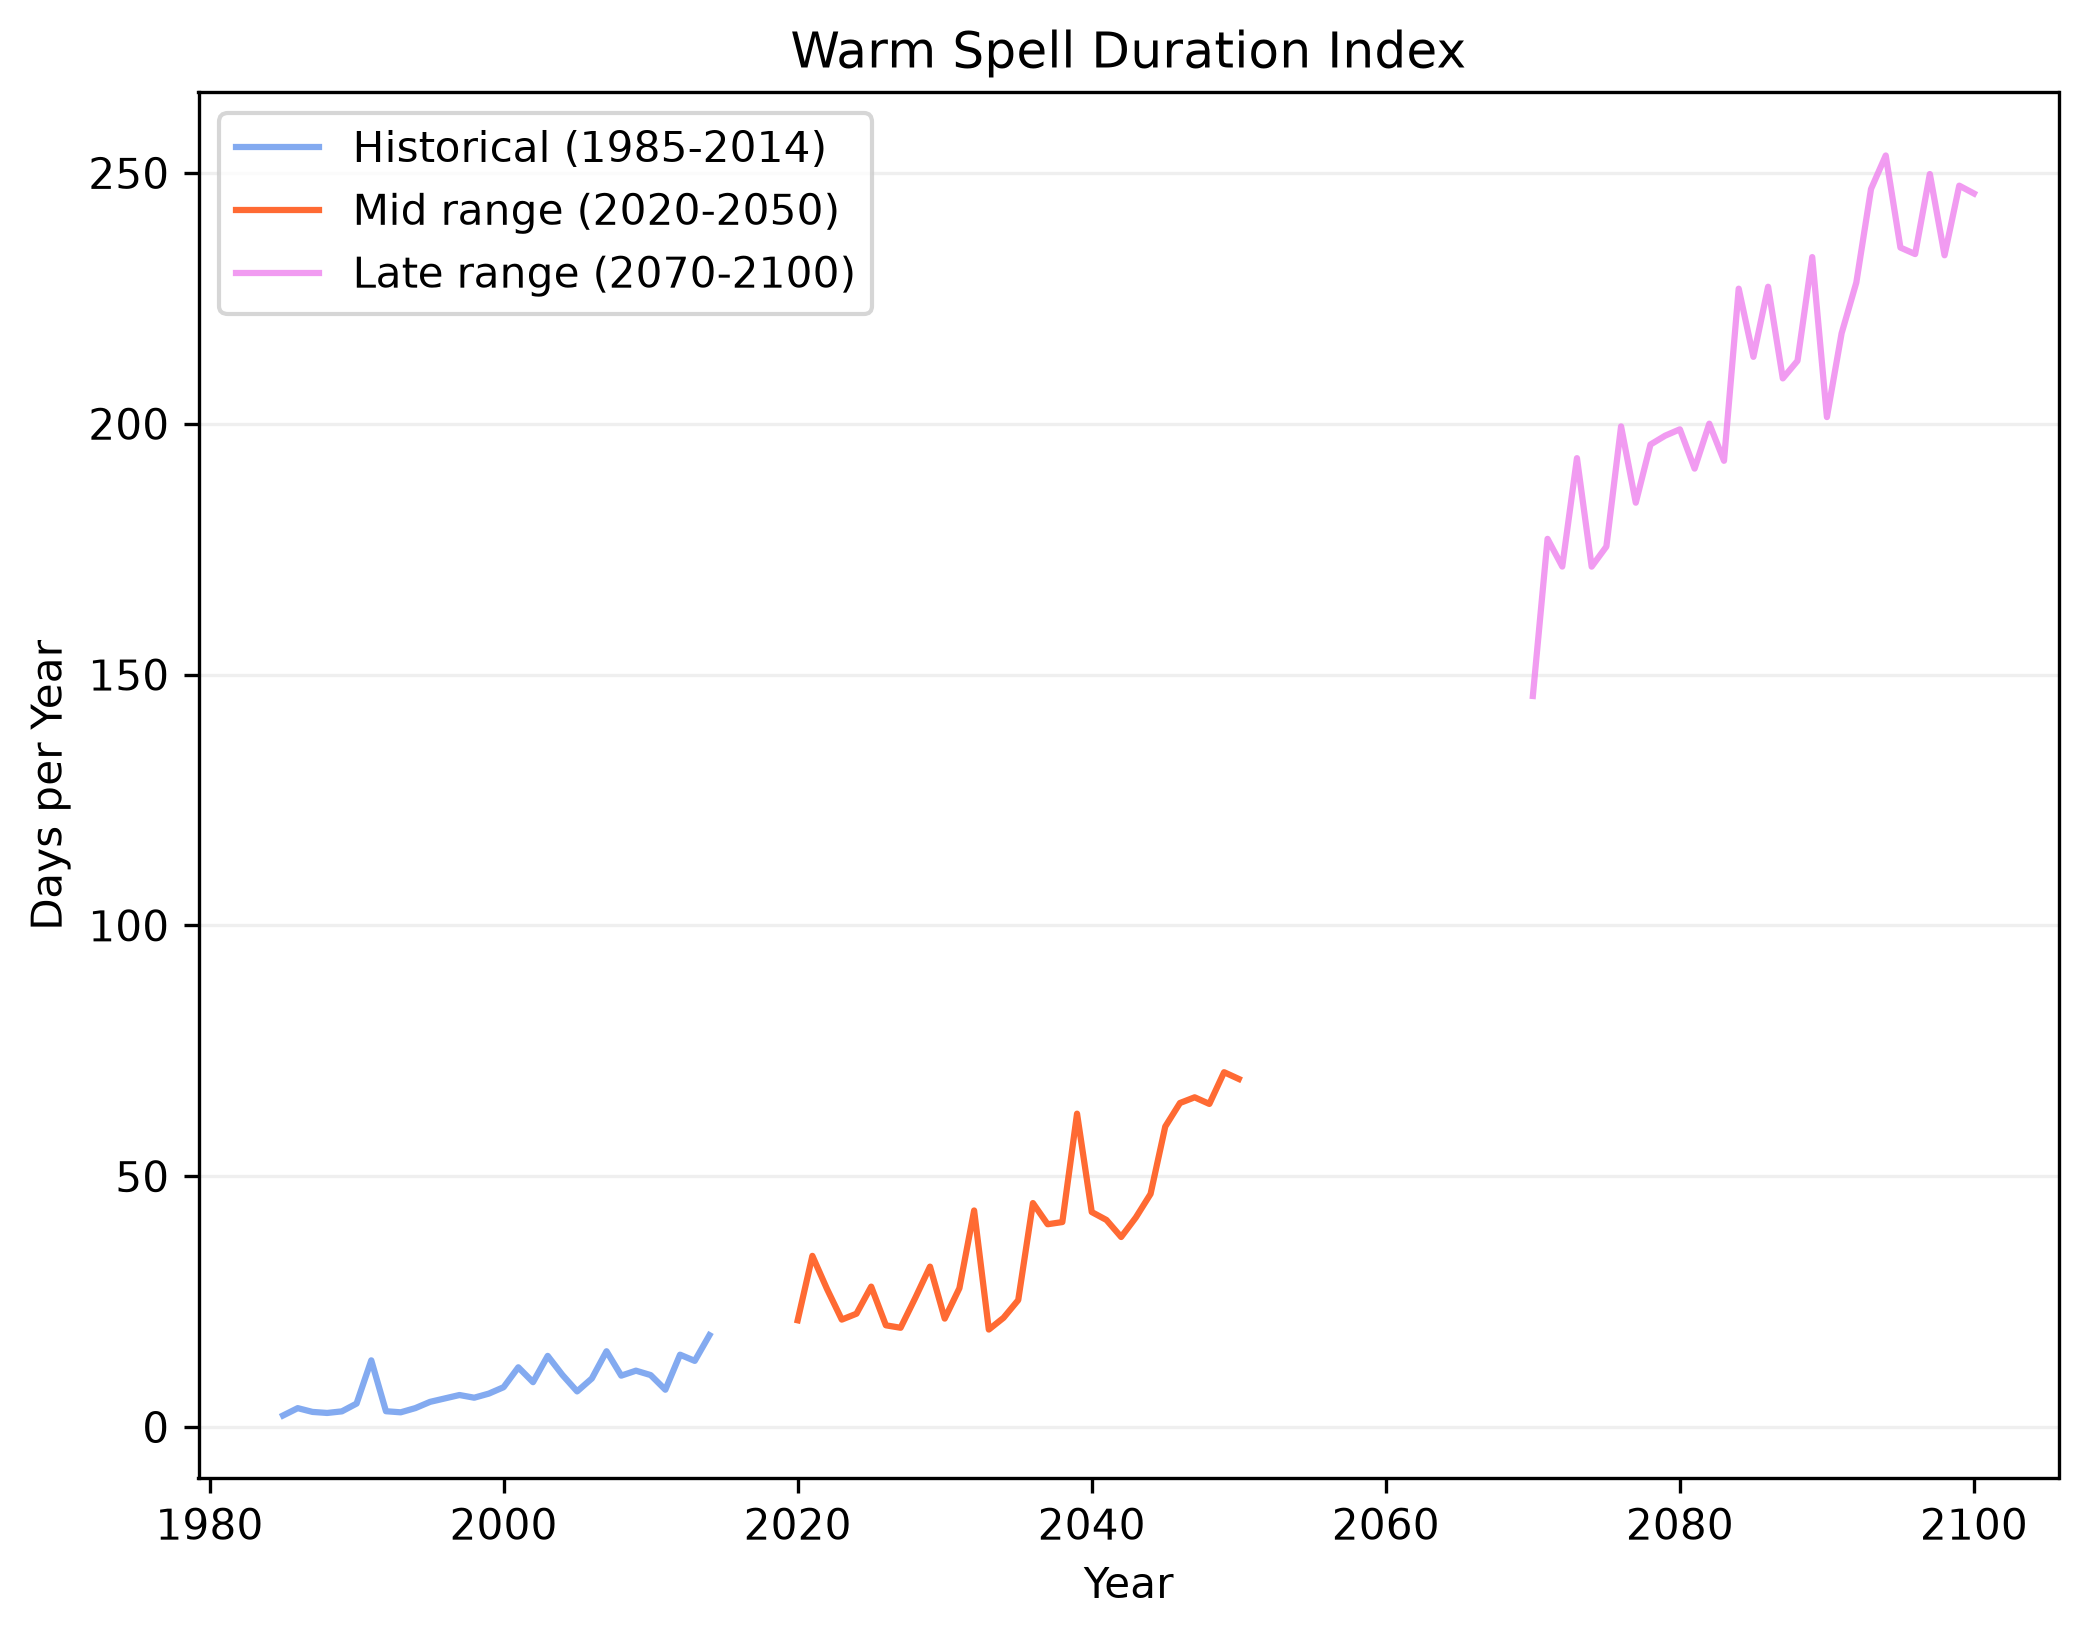
\includegraphics[width=1\linewidth]{figures/data_section/climatology/warm_spell_days_line.png}
\newpage
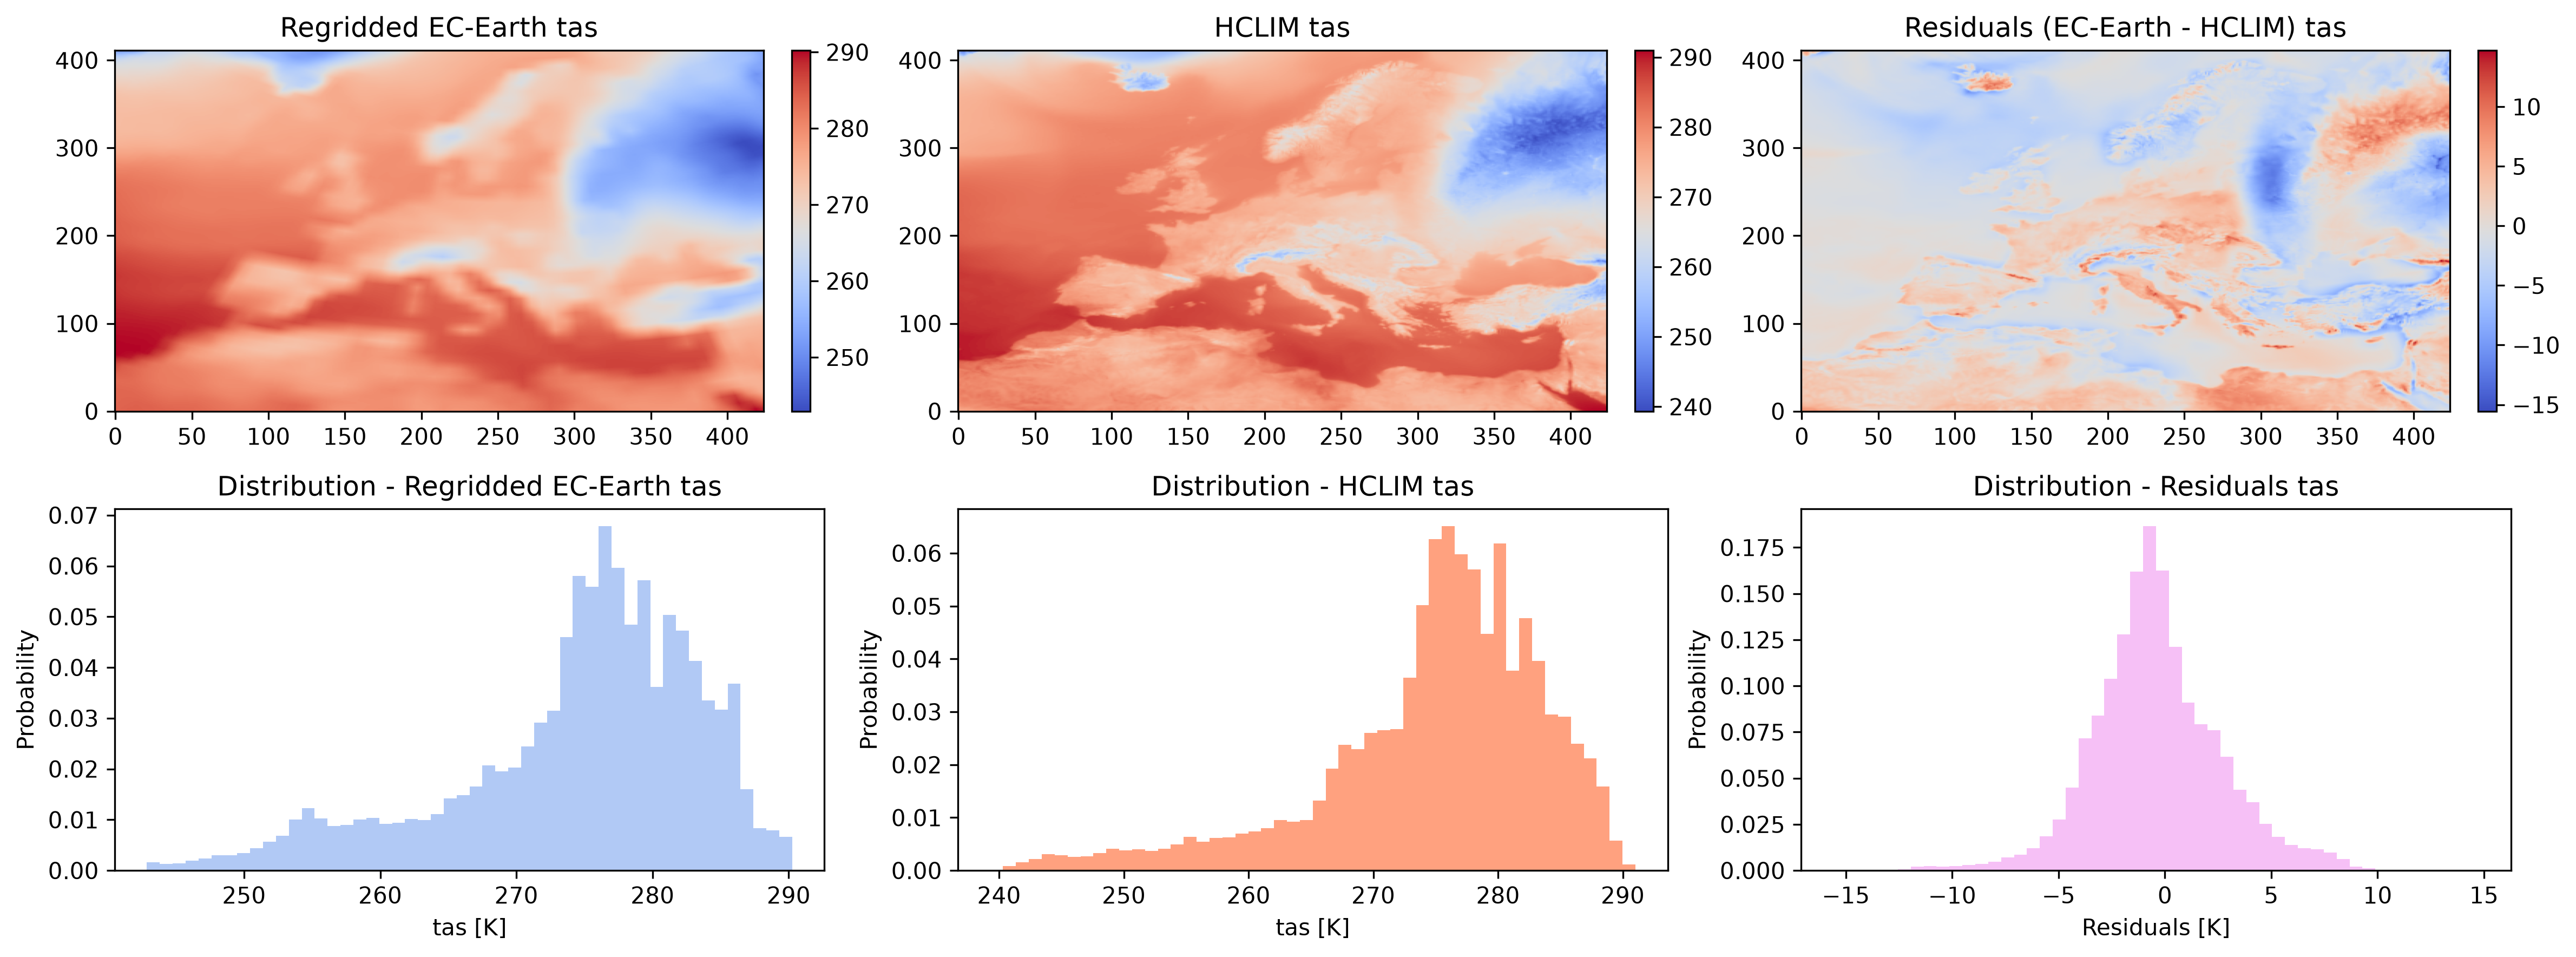
\includegraphics[width=1\linewidth]{figures/method/residuals_tas.png}
\newpage
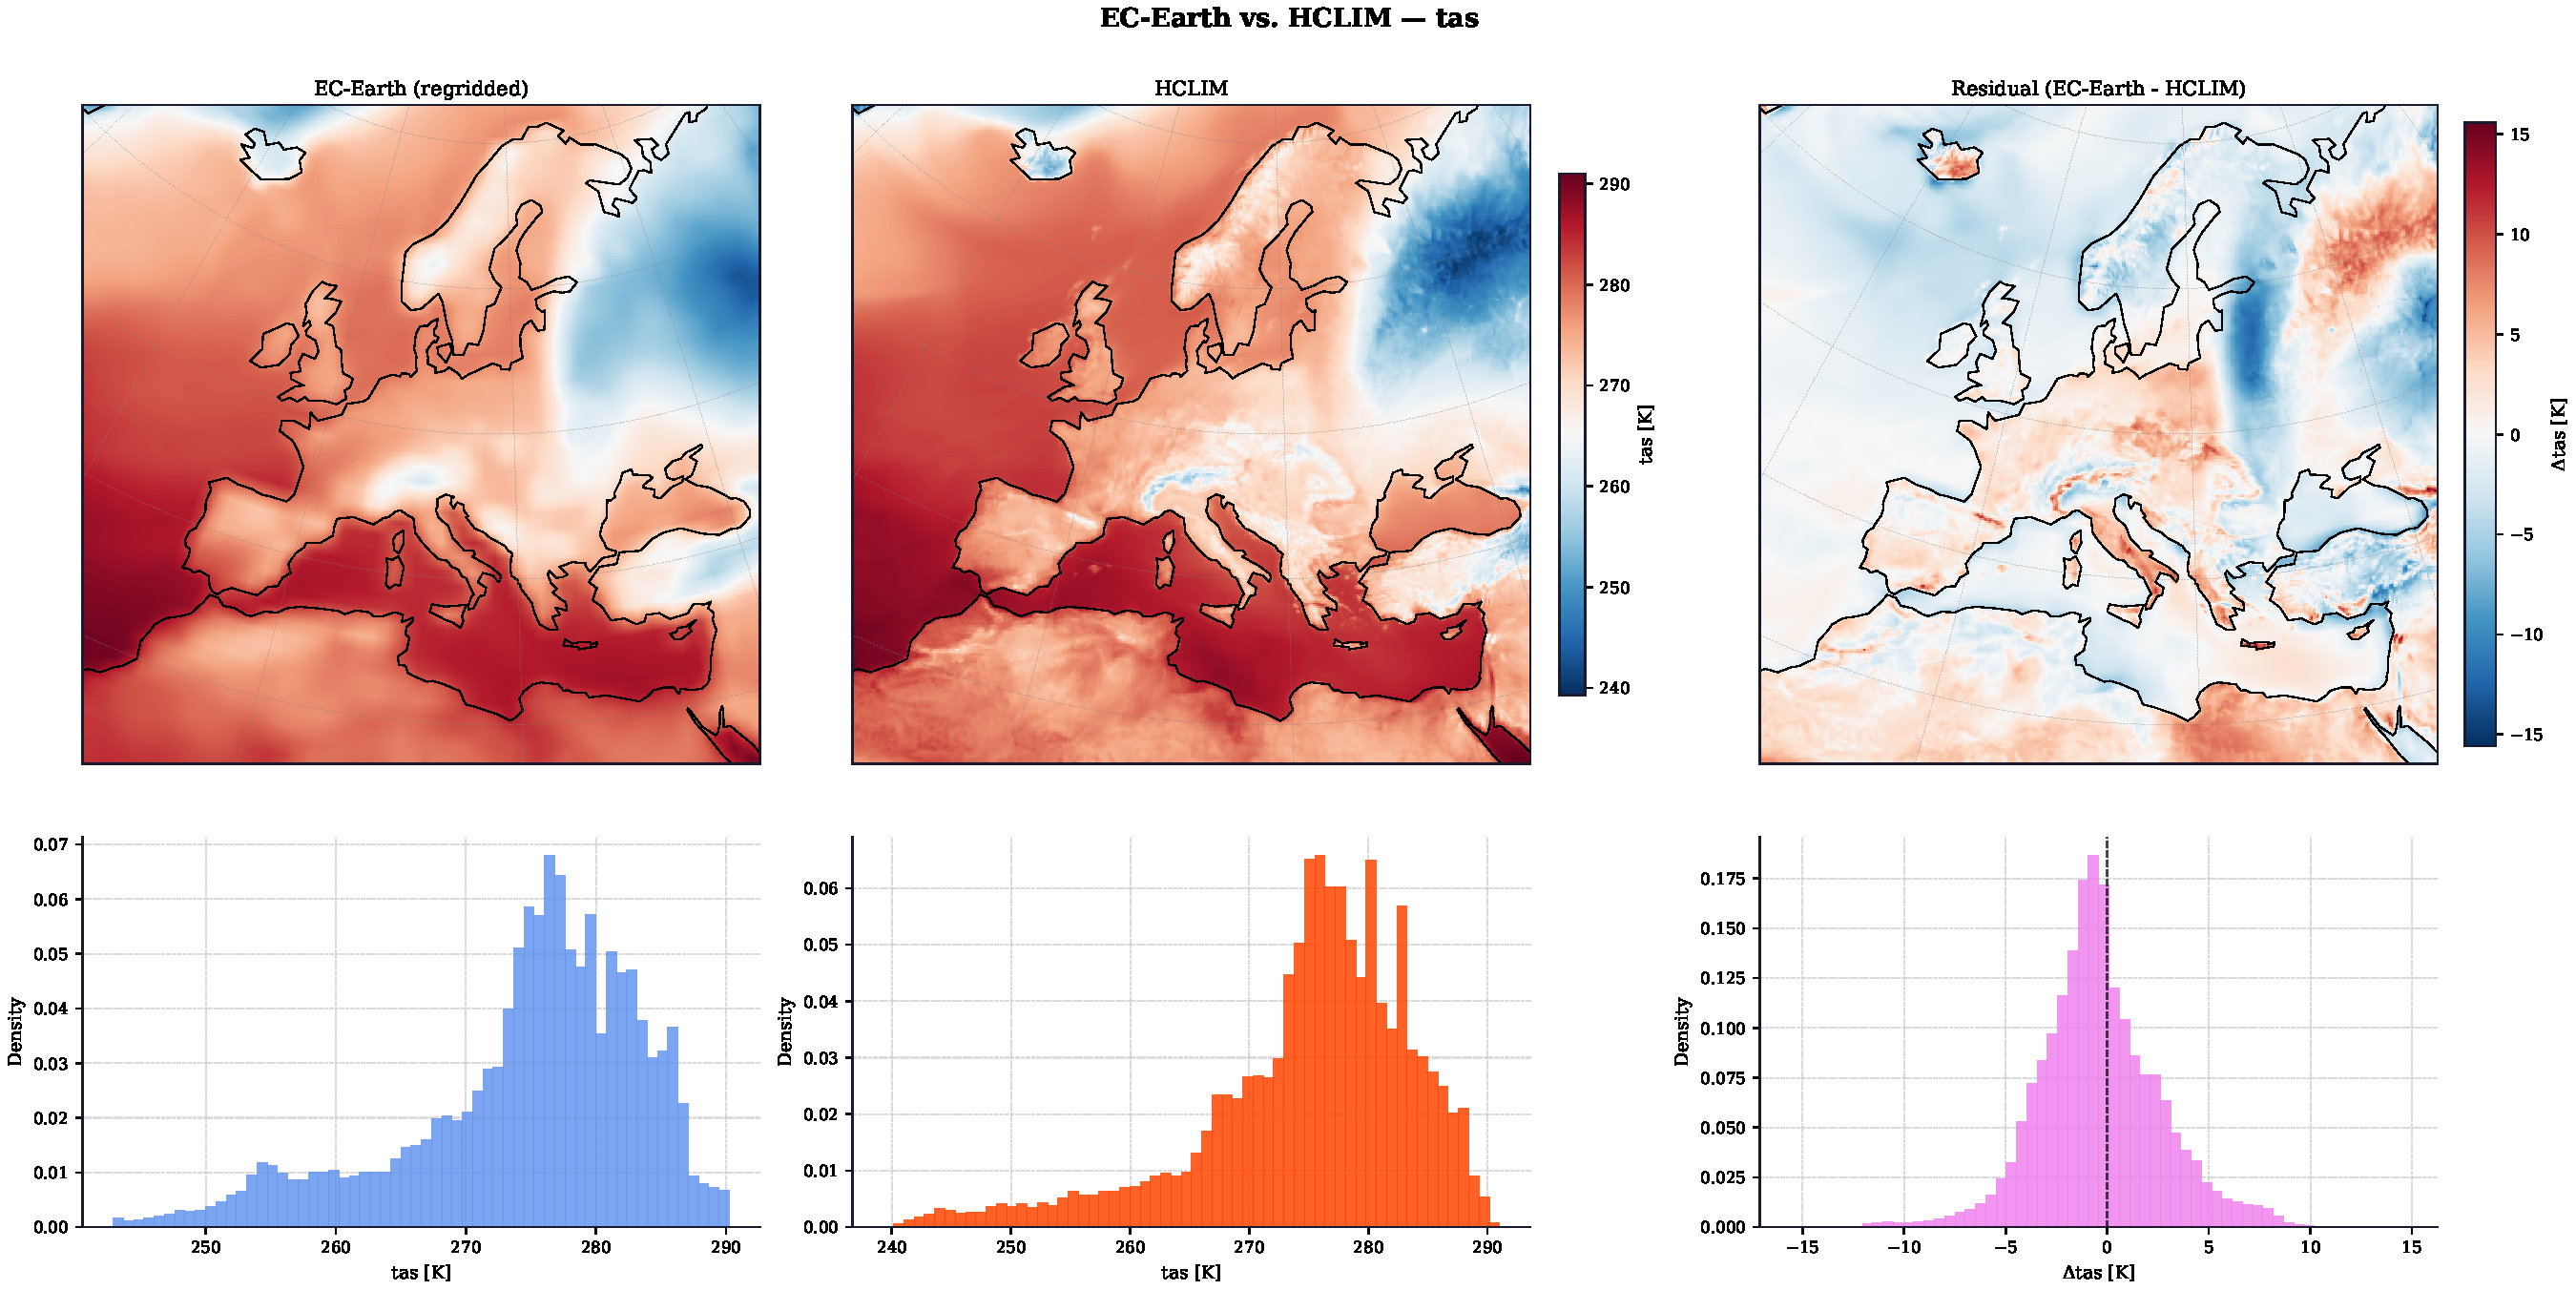
\includegraphics[width=1\linewidth]{figures/method/residuals_tas.pdf}
